\documentclass[preprint]{sigplanconf}

\usepackage{fixltx2e}

\usepackage[english]{babel}
\usepackage{amsmath,amssymb,array,listings}
\def\codefamily{\sffamily\normalsize}
\def\codesmall{\sffamily\small}

\usepackage{xspace}
\usepackage{graphicx}
\usepackage{subcaption}
\usepackage{todonotes}

\usepackage{framed}

\usepackage{xcolor}

\usepackage{tikz}
\usetikzlibrary{positioning,fit}
\usetikzlibrary{shapes.geometric}

\def\clash{C$\lambda$aSH\xspace}

\DeclareMathOperator*{\argmin}{\arg\!\min} % argmin operator

\bibliographystyle{abbrvnat}

\begin{document}
\lstset{language=Haskell, basewidth=1.2ex, basicstyle=\codefamily, identifierstyle=\itshape,
 deletekeywords={String,Maybe,Just,Nothing,map,mapM,split,bracket,when,Bool,Int,div,round,sin,maxBound,fromIntegral,odd,True,False,Eq,negate,Double,Enum,index,fromEnum,not,accum,Functor,min,max,next,lookup,const,transpose,sum,sqrt,zip,zipWith,replicate,undefined,splitAt,length,foldl1,Float,otherwise}} 

\title{Transforming Programs into Application Specific Processors}
\authorinfo{Arjan~Boeijink \and Hendrik Folmer \and Jan~Kuper \and Marco J.G. Bekooij}{University of Twente}{\{w.a.boeijink,h.h.folmer\}@utwente.nl}

\maketitle

\begin{abstract}
The combination of performance and energy efficiency drives hardware designers to create specialized components for specific applications.
Current hardware technology has the space for complex algorithms to be mapped to hardware, however this complexity makes a manual hardware design process no longer tenable.
This paper shows that implementing a program as a specialised hardware design can be a systematic process using classic compiler techniques, and yields a processors-like architecture.
From programs written in an embedded Haskell DSL with explicit clock cycle boundaries we automatically generate a synthesizable hardware descriptions for application specific processors.
\end{abstract}


\section{Introduction}
The past decades we received hardware performance gains first from higher clock frequencies and later from increased parallelism.
The energy costs (from data centers to mobile devices) are now the main bottleneck in computing, thus raising clock frequencies is no longer an option.
And exploiting more parallelism is getting harder with diminishing returns.
This leaves specialisation of hardware designs as the key method to gain effiency and performance.

The amount of logic gates avaible on a chip is still increasing, allowing complex algorithm to be directly implemented in hardware.
However the costs of producing a high performance chips with the leading edge technology has grown to the point where only few companies have the scale to design new ones.
And GPUs, while offering much parallel computation throughput, are not always suitable because of their energy consumption, and have latencies too big for real time applications.

The availability of large reconfigurable hardware chips, known as field-programmable gate arrays (FPGA), provides the opportunity to apply hardware design to many specialised applications.
Users of FPGAs range from datacenters requiring energy efficiency and fast response times, to high performance sensor data processing on a flying drone.
The complexity of algorithms to be mapped onto FPGAs and fast changing requirements of specialised applications, makes the manual hardware design process the bottleneck in time and costs.

As functional programmers we were frustrated by the low level nature of common hardware design tools and languages, and how repetitive most of hardware design process is.
Thus we are looking for higher level (and functional) abstractions for describing hardware, and to explore and bridge the gap between software and hardware.

%FPGAs became large enough for many applications.
%FPGAs even available as accelerators for cloud computing.

%From the outside hardware is usually a small black box with number of pins connected to it.
%The inside a of chip consists of a large numbers of transistors are connected by wires.

% Some questions after reflecting on my own research:
%\begin{itemize}
% \item What is the real difference between software and hardware?
% \item Why seems instruction set design obvious in hindsight?
%% \item What are the important choices in ISA/processor design?
%% \item How to make processor design a more systematic process?
%\end{itemize}

In the first part of this paper we show a systematic transformation process of a functional program into a simple processor using well known techniques and some hardware oriented optimisations.
Next we apply this concept of application specific processor generation to a practical useful setting.
An embedded Haskell DSL with explicit clock cycle boundaries is introduced, which gives the hardware designer a lot control over the generated hardware implementation.
With a tool to generate \clash code from this DSL, we keep the whole hardware design process in Haskell with executable/simulatable code at every stage.
As a demonstration application we use the hardware implementation on an FPGA of the signal processing for a laser range finder.


\subsection{Background: a Haskell based hardware design process}
Functional languages have a long history with hardware design \cite{Sheeran2005}.
A hardware design process in Haskell using \clash is described in \cite{Robin:Hendrik} and contains the following steps:
The first step is to choose an algorithm to solve the a certain problem.
While choosing an algorithm it is important to keep in mind how well the target hardware could potentially solve the problem.
FPGAs are suitable for reusing computational structures and consistent data streams.
The next step is to specify the algorithm in executable Haskell code. After which the code can be rewritten in executable \clash -code.
The functionality can be evaluated/simulated in the Haskell/\clash. The \clash compiler can automatically generate a hardware architecture which can be synthesized to determine the hardware resource costs.
The synthesized architecture consumes a certain amount of hardware resources but the target device has a limited amount of resources available.
These resource constrains are in terms of memory, memory bandwidth, logical elements, and digital signal processors (DSPs).
There are also constrains on latency and throughput. There are several methods to create a feasible design for the given resource constrains. One could split the algorithm in steps to reduce data access to limit the memory bandwidth.
Finding patterns in the algorithm allows for the reuse of hardware components over time.
This limits both memory and computational area on an FPGA. Breaking long latency computation in parts enable faster clock frequencies which influences latency and throughput.
Pipelining and multistep computation requires glue logic/control to operate.
During the time-area trade-off one can iterate through all the above mentioned methods. 

The nice aspect of this process is that every step the result can be evaluated/simulated because it is executable Haskell/\clash code.
In the time-area trade-off  the impact of every design choice can be evaluated. The downside of this method, especially when iteratively designing a time-area trade-off, is that it comes down to the designers knowledge which technique is necessary to make a feasible design.

Creating glue logic and control to operate the algorithm is error prone and requires the majority of the effort.
The automation of this part of the process is the main goal of this paper.
% This paper presents a method of deducing the control- and data-path from the algorithm, given the algorithms execution order??

\subsection{Hardware in Haskell using \clash}
Designing hardware architectures for FPGA is traditionally done using low-level hardware description languages (HDLs) like Verilog or VHDL which is cumbersome and prone to error. \clash 
\clash \cite{Baaij} is a subset of Haskell that can be compiled to widely supported lower level HDLs.
Even though you can use most abstractions that Haskell has to offer, \clash is still a structural hardware description language.
Being a structural hardware description language \clash does not support dynamic data sizes or recursion, so in order to convert Haskell to \clash one has to use fixed size vectors instead of lists, specify the size of value data, and use higher-order functions or mealy machine structures instead of recursion.

%\subsection{Hardware in Haskell using \clash}
%\subsection{The hardware design process in practice}
%\begin{enumerate}
% \item Choose algorithm
% \item Convert math/pseudo code to executable Haskell
% \item fixed size vectors
% \item select numeric precision
% \item synthesize for hardware resource costs
% \item split algorithm in steps to reduce data access to feasible memory bandwith
% \item find patterns in algorithm to enable reuse of hardware components
% \item break long latency computation in parts to enable good clock frequencies
% \item write glue logic/control for pipelining and multistep computations
% \item synthesize design for target hardware platform
% \item iterate parts of this process until satisfied with performance/costs
%\end{enumerate}
%The nice aspect of this process is that every refinement of the design is described as executable haskell code.
%Thus you can easily compare outputs of each step and see the impact of design choices on precission.
%The downside is that you often come to conclusion that the algoritm choosen doesn't achieve the performance/costs you want. So you have to go through all steps again.
%Steps 6 to 9 take the most effort, and step 9 is very error prone and can be very complex.

\section{Rewriting a program into a processor}
As a running example in this section we use a binary variant of greatest common divisor, that doesn't use any complex arithmetic operation.
The use of multiple recursive functions and a data dependent recursion depth makes it non trivial to implement this computation in hardware.
\begin{lstlisting}
binGCD :: Word32 -> Word32 -> Word32       
binGCD x 0 = x
binGCD x y = let
    a = dropZeros x
    b = dropZeros y
    (s,g) = (min a b, max a b)
  in binGCD s (g - s) <<< countZeros (x .|. y)

dropZeros :: Word32 -> Word32
dropZeros i = i >>> countZeros i

countZeros :: Word32 -> Word32
countZeros n = if odd n then 0 
  else countZeros (n >>> 1) + 1
\end{lstlisting}
The count trailing zeros could been implemented as a primitive operation as a fold over bits.

\subsection{Desugaring and flattening the program}
The first step is splitting up expressions which are too complex to execute within a single clock cycle.
This can be done by introducing let expression like in the conversion to administrative normal form \cite{ANF}.
The question is, which expressions to define as trivial, as for example some arithmetic operations mights be cheap enough to keep nested.
For this example we will split up all nested expression, in order to produce a very simple processor.
\begin{lstlisting}
binGCD x y = 
  if (y == 0) then x
  else
    let a = dropZeros x in
    let b = dropZeros y in
    let g = max a b in
    let s = min a b in
    let d = g - s in
    let r = binGCD s d in
    let o = x .|. y in
    let e = countZeros o in
    r <<< e
\end{lstlisting}

\subsection{Explicit sequential execution}
Making control flow explicit using continuation passing style \cite{AppelCwC} is a standard method in compilers for functional languages.
With an already flattened program we only have to introduce a continuation for the body of each let expression:
\begin{lstlisting}
binGCD x y k = if (y == 0)
  then cont x k
  else
    dropZeros x
      (\a -> dropZeros y
        (\b -> cont (max a b)
          (\g -> cont (min a b)
            (\s -> cont (g - s)
              (\d -> binGCD s d
                (\r -> cont (x .|. y)
                  (\o -> countZeros o
                    (\e -> cont (r <<< e) k)
      )))))))
\end{lstlisting}
Here we use the $cont$ function to make continuation application explicit. \\

\textit{To add a bit more information for those not familar with CPS}

\subsection{Defunctionalising continuations}
Defunctionalisation \cite{Reynolds} is well known technique to transform functions into datatypes. \\

\textit{Explanation to be added here}

\lstset{basicstyle=\codesmall}
\begin{lstlisting}
data Cont
  = CA Word32 Word32                      Cont
  | CB Word32 Word32 Word32               Cont
  | CC Word32 Word32 Word32 Word32        Cont
  | CD Word32 Word32 Word32 Word32 Word32 Cont

binGCD x y         k  = if (y == 0)
                   then cont x         k
                   else dropZeros x    (CA x y       k)
cont a (CA x y     k) = dropZeros y    (CB x y a     k)
cont b (CB x y a   k) = cont (max a b) (CC x y a b   k)
cont g (CC x y a b k) = cont (min a b) (CD x y a b g k)
\end{lstlisting}
\lstset{basicstyle=\codefamily}

The steps of continuation passing style and defunctionalisation could be combined into one as shown in 'Calculating Correct Compilers'\cite{CCC}.


\subsection{State machine with a stack}
Here we apply the tranformation from translating recursive functions to hardware in \cite{Ingmar} and \cite{Zhai}.

Using the observation that nested continuations form a stack, the nested continuation datatype can be flattened context dataype.
And we can combine functions into one by making each a data type, including the continuation application function. \\

\textit{To be explained, this key step in the process}

\begin{lstlisting}
data Call = GCD Word32 Word32 | DropZs Word32
          | CntZs Word32 | Cont Word32
data Context
  = CA Word32 Word32
  | CB Word32 Word32 Word32
  | CC Word32 Word32 Word32 Word32
  | CD Word32 Word32 Word32 Word32 Word32
  ...
type Stack  = [Context]

step :: Call -> Stack -> (Call, Stack)
step (GCD x y)        cs = if y == 0
  then (Cont x      , cs               )
  else (DropZs x    , CA x y       : cs)
step (Cont a)        (CA x y       : cs) =
     (DropZs y      , CB x y a     : cs)
step (Cont b)        (CB x y a     : cs) =
     (Cont (max a b), CC x y a b   : cs)
step (Cont g)        (CC x y a b   : cs) =
     (Cont (min a b), CD x y a b g : cs)
\end{lstlisting}

\begin{figure}
\centering
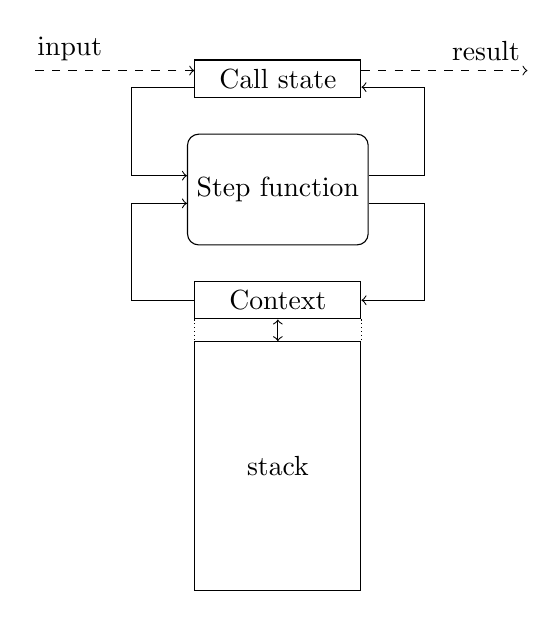
\begin{tikzpicture}
\node[draw, shape=rectangle, minimum width=6em] (st) {Call state};
\node[draw, shape=rectangle, minimum width=6em, minimum height=4em, below of=st, node distance=4em, rounded corners] (fun) {Step function};
\node[draw, shape=rectangle, minimum width=6em, below of=fun, node distance=4em] (con) {Context};
\node[draw, shape=rectangle, minimum width=6em, minimum height=9em, below of=con, node distance=6em] (ck) {stack};
\draw[densely dotted] (con.south west) -- (ck.north west);
\draw[densely dotted] (con.south east) -- (ck.north east);
\draw[->, dashed] ([yshift=0.3em]st.east) -- node[above, near end] {result} ([yshift=0.3em,xshift=6em]st.east);
\draw[<-, dashed] ([yshift=0.3em]st.west) -- node[above, near end] {input} ([yshift=0.3em,xshift=-6em]st.west);
\draw[->] ([yshift=0.5em]fun.east) -| ([xshift=2em]fun.north east) |- ([yshift=-0.3em]st.east);
\draw[->] ([yshift=-0.3em]st.west) -| ([xshift=-2em]fun.north west) |- ([yshift=0.5em]fun.west);
\draw[->] ([yshift=-0.5em]fun.east) -| ([xshift=2em]fun.south east) |- (con.east);
\draw[->] (con.west) -| ([xshift=-2em]fun.south west) |- ([yshift=-0.5em]fun.west);
\draw[<->] (con.south) -- (ck.north);
\end{tikzpicture}
\caption{Hardware structure of the stack machine}
\label{fig:stack}
\end{figure}
Figure \ref{fig:stack} shows the stack machine structure as hardware

\subsection{Separating the data stack}
Most steps have a lot of data copied from one continuation to another, and stack is very wide because some continuations capture many free variables.
This yield inefficient hardware, especially when only a few variables are used every cycle. \\

\textit{To explain the transformation here}

\begin{lstlisting}
data State = BinGCD | DropZs | CntZs | Cont
data Context = CA | CB | CC | CD | ...
type CtrlStack  = [Context]
type DataStack = [Word32]

step ::  State -> CtrlStack -> DataStack ->
  (State, CtrlStack, DataStack)
step BinGCD     cs      (y:x:ds) = if y == 0
  then (Cont  , cs   ,     x:ds)
  else (DropZs, CA:cs, x:y:x:ds)
step Cont (CA:cs)     (a:y:x:ds) = 
  (DropZs, CB:cs,    y:a:y:x:ds)
step Cont (CB:cs)   (b:a:y:x:ds) = 
  (Cont,   CC:cs,  g:b:a:y:x:ds) where g = max a b
step Cont (CC:cs) (g:b:a:y:x:ds) = 
  (Cont,  CD:cs, s:g:b:a:y:x:ds) where s = min a b
\end{lstlisting}
Note that we have to copy the argument to the dropZeros function because they are used again and/or in the wrong order.
And for the arguments to the recursive binGCD call we can skip copying as they are in the right order and not used later.

Having two stacks might look like a unnecessary complication from the C-like software stack point of view, but is common in hardware designs based on Forth \cite{LaForest}.

\subsection{Optimizing control}
What happens in every step depends on both the state and top of the continuation stack.
We can combine the control state and continuation stack into a control stack by eliminating the Return state.
Then only the top of the control stack directly determines what each step does.
The steps containing if expressions are more complex than the rest, and can be split up by computing the branch condition in a separate step.

\begin{lstlisting}
data Label = BinGCD | T1 | E1 | CA | CB | CC
   | CDE | DropZs | ... deriving Enum
type ControlStack  = [Label]
type DataStack = [Word32]
type CtrlFun = Label -> CtrlStack -> 
  (Label, CtrlStack)

step :: Label -> DataStack -> (CtrlFun,DataStack)
step BinGCD        (y:x:ds) =
  (branch E1 z,     y:x:ds) where z = y == 0
step T1            (y:x:ds) = 
  (ret        ,       x:ds)
step E1            (y:x:ds) = 
  (call DropZs,   x:y:x:ds)
step CA          (a:y:x:ds) = 
  (call DropZs, y:a:y:x:ds)
step CB        (b:a:y:x:ds) = 
  (next     , g:b:a:y:x:ds) where g = max a b
step CC      (g:b:a:y:x:ds) = 
  (next   , s:g:b:a:y:x:ds) where s = min a b
\end{lstlisting}

Now we can recognise the top of the control stack as a program counter.
Thus a program counter is merely a numeric encoded label, optimized for the common case of continuing at the successive label.

The resulting dual stack machine looks like something you could derive directly by looking at the flattened program from tradition imperative language point of view.

\subsection{Splitting into components}
To be able to use efficient existing memory components we have to extract the use of the datastack from the step function.
This means splitting each step in parts to separate memory read and write actions.
Also splitting off the arithmetic operations makes it easier to reuse hardware for similar (arithmetic) computations.

\begin{lstlisting}
type CtrlFun = Word32 -> Label -> CtrlStack ->
   (Label, CtrlStack)
type Input = DataStack -> Word32
type AluOp = Word32 -> Word32 -> Word32
type StackMod = Word32 -> DataStack -> DataStack
\end{lstlisting}

\lstset{basicstyle=\codesmall}
\begin{lstlisting}
step :: Label -> (CtrlFun,Input,Input,AluOp,StackMod)
step GCD = (branch E1  ,peek 0,lit 0 , isEq ,keep)
step T1  = (ret        ,peek 1,lit 0 , pass ,popNPush 2)
step E1  = (call DropZs,peek 1,lit 0 , pass ,push)
step CA  = (call DropZs,peek 1,lit 0 , pass ,push)
step CB  = (next       ,peek 1,peek 0, max  ,push)
step CC  = (next       ,peek 2,peek 1, min  ,push)
\end{lstlisting}
\lstset{basicstyle=\codefamily}

[TODO] check if such a description would be synthesizable in \clash{}

\subsection{Control by microcode}
Each step is now defined as a set of functions to be executed, however functions can not directly exist in hardware.
Thus we apply defunctionalisation to each aspect, yielding components controlled by datatypes.
The resulting structure looks like a processor controlled by horizontal microcode.

\begin{lstlisting}
data AluOp = Const | Add | Sub | Or | Min | Max |
   ShR | ShL | IsEq | IsOdd
data Input = S Int | I Word32
data StAction = Keep | Push | PopNPush Int
data Ctrl = Call Label |Return |Branch Label |Next
\end{lstlisting}

\lstset{basicstyle=\codesmall}
\begin{lstlisting}
microcode :: Label -> (Ctrl,Input,Input,AluOp,StAction)
microcode pc = case pc of
  BinGCD -> (Branch E1  , S 0, I 0, IsEq , Keep)
  T1     -> (Return     , S 1, I 0, Pass , PopNPush 2)
  E1     -> (Call DropZs, S 1, I 0, Pass , Push)
  CA     -> (Call DropZs, S 1, I 0, Pass , Push)
  CB     -> (Next       , S 1, S 0, Max  , Push)
  CC     -> (Next       , S 2, S 1, Min  , Push)
  CDE    -> (Call BinGCD, S 1, S 0, Sub  , Push)
  CFG    -> (Call CntZs , S 5, S 4, Or   , Push)
  CH     -> (Return     , S 1, S 0, ShL  , PopNPush 7)
  DropZs -> (Call CntZs , S 0, I 0, Pass , Push)
  CI     -> (Return     , S 1, S 0, ShR  , PopNPush 2)
  CntZs  -> (Branch E2  , S 0, I 0, IsOdd, Keep)
  T2     -> (Return     , I 0, I 0, Pass , PopNPush 1)
  E2     -> (Call CntZs , S 0, I 1, ShR  , Push)
  CK     -> (Return     , S 0, I 1, Add  , PopNPush 2)
\end{lstlisting}
\lstset{basicstyle=\codefamily}

\begin{lstlisting}
alu :: AluOp -> Word32 -> Word32 -> Word32
alu Pass  x _ = x
alu Add   x y = x + y
alu Sub   x y = x - y
alu Or    x y = x .|. y
alu Min   x y = min x y
alu Max   x y = max x y
alu ShR   x y = x >>> y
alu ShL   x y = x <<< y
alu IsEq  x y = if x == y then 1 else 0
alu IsOdd x _ = if odd x then 1 else 0

selInput :: DataStack -> Input -> Word32
selInput ds (S i) = ds !! i
selInput _  (I x) = x

stackMod :: StAction -> Word32 -> 
  DataStack -> DataStack
stackMod Keep             = keep
stackMod Push             = push
stackMod (PushAfterPop n) = pushAfterPop n

ctrl :: Ctrl -> Word32 -> Label -> [Label] ->
  (Label, [Label])
ctrl Next       = next
ctrl Return     = ret
ctrl (Branch e) = branch e
ctrl (Call f  ) = call f
\end{lstlisting}

\subsection{Synthesisable implementation in \clash}
The main effort of converting into a synthesisable hardware description is in replacing the lists for the control and data stack with memory components and stack pointers.
Both stack pointers and the program counter need to be stored in a register.
The $microcode$ and $alu$ code from previous step can be directly reused with any change.
All components are then connected together in the toplevel of the processor description.
This is straightforward except for having to work with Applicative glue logic for Signal's instead of pure values

\begin{lstlisting}
proccesor :: Signal () -> Signal (Label, Word32)
proccesor _ = bundle (pc, z) where
  pc = register def pc'
  (ctrlOp,ia,ib,oper,stOp) = liftB microcode pc

  nPC = liftA succ pc
  (cSP', savePC, pc') = 
    liftB5 ctrl ctrlOp z nPC cSP retPC
  cSP = register 0 cSP'
  retPC = asyncRam d64 cSP savePC

  rdA = liftA2 agu dSP ia
  rdB = liftA2 agu dSP ib
  a = asyncRam d128 rdA wrData
  b = asyncRam d128 rdB wrData

  x = liftA2 inputMux ia a
  y = liftA2 inputMux ib b
  z = liftA3 alu oper x y

  dSP = register 0 dSP'
  (dSP', wrData) = liftB3 stackMod stOp dSP z
\end{lstlisting}

\begin{lstlisting}
agu :: Word8 -> Input -> Word8
agu stackSp (S i) = stackSp - i
agu stackSp (I _) = stackSp

ctrl :: Ctrl -> Word32 -> Label -> Word8 -> Label
  -> (Word8, Maybe (Word8, Label), Label)
ctrl Next       _ nPC cSP retPC =
  (cSP  , Nothing          , nPC)
ctrl Return     _ nPC cSP retPC =
  (cSP-1, Nothing          , retPC)
ctrl (Branch e) 0 nPC cSP retPC =
 (cSP  , Nothing          , e)
ctrl (Branch e) _ nPC cSP retPC =
  (cSP  , Nothing          , nPC)
ctrl (Call f)   _ nPC cSP retPC =
  (cSP+1, Just (cSP+1, nPC), f)

stackMod :: StAction -> Word8 -> Word32 ->
  (Word8, Maybe (Word8, Word32))
stackMod Keep         dSP z =
  (dSP , Nothing)
stackMod Push         dSP z =
  (dSP', Just (dSP', z)) where dSP' = dSP+1
stackMod (PopNPush n) dSP z =
  (dSP', Just (dSP', z)) where dSP' = dSP-n+1
\end{lstlisting}

\begin{figure}
\centering
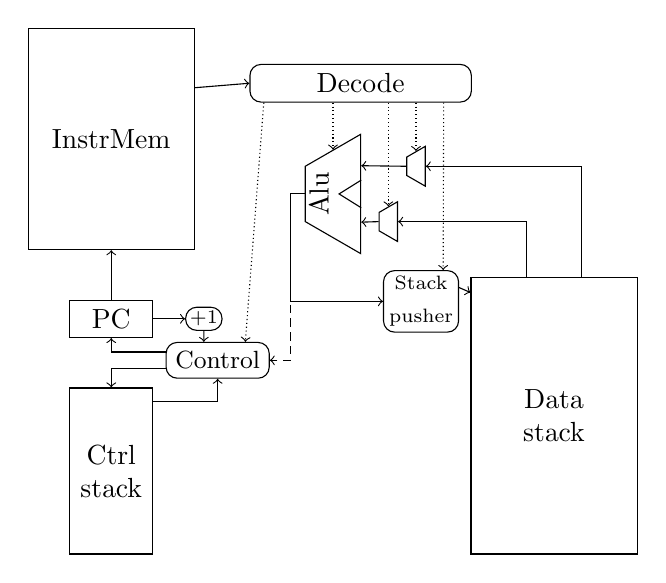
\begin{tikzpicture}
\node[draw, shape=rectangle, minimum width=6em, minimum height=8em] (im) {InstrMem};
\node[draw, shape=rectangle, rounded corners, minimum width=8em, above right of=im, xshift=7em] (dec) {Decode};
\node[draw, shape=rectangle, minimum width=3em, below of=im, node distance=6.5em] (pc) {PC};
\node[draw, shape=rectangle, rounded corners, right of=pc, xshift=0.5em, inner sep=0.15em] (npc) {\begin{scriptsize}$+1$\end{scriptsize}};
\node[draw, shape=rectangle, rounded corners, right of=pc, xshift=1em, yshift=-1.5em] (cc) {\begin{small}Control\end{small}};
\node[draw, shape=rectangle, minimum width=3em, minimum height=6em, below of=pc, node distance=5.5em, align=center] (cs) {Ctrl\\stack};
\node[draw, shape=rectangle, minimum width=6em, minimum height=10em, below of=im, node distance=10em, align=center, xshift=16em] (ds) {Data\\stack};
\node[draw, shape=trapezium, minimum width=3em, minimum height=2em, below of=dec, node distance=4em, xshift=-1em, rotate=90] (alu) {};
\node[xshift=-0.5em, rotate=90] at (alu.center) {Alu};
\node[draw, shape=rectangle, rounded corners, below right of=alu, node distance=4.5em, yshift=-0.7em, inner sep=0.2em, align=center] (sp) {\begin{scriptsize}Stack\end{scriptsize}\\\begin{scriptsize}pusher\end{scriptsize}};
\draw ([yshift=0.5em] alu.south) -- ([xshift=-0.8em] alu.south) -- ([yshift=-0.5em] alu.south);
\node[draw, shape=trapezium, minimum width=1em, minimum height=0.5em, right of=alu, node distance=3em, yshift=1em, rotate=90] (ina) {};
\node[draw, shape=trapezium, minimum width=1em, minimum height=0.5em, right of=alu, node distance=2em, yshift=-1em, rotate=90] (inb) {};
\draw[->] (ina.north) -- (alu.south east);
\draw[->] (inb.north) -- (alu.south west);
\draw[->] ([xshift=1em] ds.north) |- (ina.south);
\draw[->] ([xshift=-1em] ds.north) |- (inb.south);
\draw[->] (pc.north) -- (im.south);
\draw[->] (pc.east) -- (npc.west);
\draw[->] (npc.south) -- ([xshift=-0.5em] cc.north);
\draw[->] ([yshift=1.85em] im.east) -- (dec.west);
\draw[->] ([yshift=0.3em] cc.west) -| (pc.south);
\draw[->] ([yshift=-0.3em] cc.west) -| (cs.north);
\draw[->] ([yshift=2.5em]cs.east) -| (cc.south);
\draw[->] ([yshift=0.5em] sp.east) -- ([yshift=4.45em] ds.west);
\draw[->] (alu.north) -- ([xshift=-0.5em] alu.north) |- (sp.west);
\draw[->, densely dashed] (alu.north) -- ([xshift=-0.5em] alu.north) |- (cc.east);
\draw[->, densely dotted] ([xshift=-3.5em] dec.south) -- ([xshift=1em] cc.north);
\draw[->, densely dotted] ([xshift=-1em] dec.south) -- (alu.east);
\draw[->, densely dotted] ([xshift=1em] dec.south) -- (inb.east);
\draw[->, densely dotted] ([xshift=2em] dec.south) -- (ina.east);
\draw[->, densely dotted] ([xshift=3em] dec.south) -- ([xshift=0.8em]sp.north);
\end{tikzpicture}
\caption{Architecture of derived processor}
\label{fig:proc}
\end{figure}
Figure \ref{fig:proc} shows a schematic of the derived processor architecture

\subsection{Differences with general purpose processors}

The downside of using horizontal microcode is that it costs a lot of bits to encode each step in the program \\
also writing microcode by hand is a lot of work \\
thus almost all processors define an instruction set that provides a slightly higher way of writing programs \\
having instructions in a writable memory makes a processor reusable for other applications \\
from the processor point of view an instruction set is just a compressed form of microcode with a hardware component for decoding (decompressing) \\
secondly an instruction set gives the opportunity of improving the next generation of a processor design without having to change all software

\begin{lstlisting}
instrMem :: [(Label, Instr)]
decode :: Instr->(Input,Input,Oper,StAction,Ctrl)

selInput :: DataStack -> Input -> Word32
alu :: Oper -> Word32 -> Word32 -> Word32
stackMod :: StAction->Word32->DataStack->DataStack
ctrl :: Ctrl -> Word32 -> CtrlStack -> CtrlStack

sim :: DataStack -> [Label] -> Word32
sim ds []       = top ds
sim ds (pc:cs) = sim ds' cs' where
  Just is = P.lookup pc instrMem
  (ia, ib, op, g, f) = decode is
  x = selInput ds ia
  y = selInput ds ib
  z = alu op x y 
  ds' = stackMod g z ds
  cs' = ctrl f z (pc : cs)
\end{lstlisting}

\textit{TODO heap memory, pipelining and input/ouput }

\section{A DSL for explicitly clocked programs}
When designing application specific hardware components we care a lot about performance and/or efficiency, otherwise we could have used some existing processor.
The gains come from doing some specialised computation in less steps (clock cycles) and/or doing more operations in parallel than a normal processor could.
While the transformation process described in previous produces a working processor, it is fairly minimalistic and not that efficient.
The decision of how much computation to do in each step is a complex optimisation problem that depends on area and clock frequency requirements.
Thus we leave it up to the hardware designer to explicitly decide how to group computations into clock cycles.
Also the timing with respect to other components can be important, so the order of execution of each cycle needs to be explicit.

\subsection{The sequential logic monad}

\textit{To be explained}

\subsection{Expressing control flow}
Using functions is essential for code reuse and readability of larger programs, thus multi cycle SeqLogic fragments should be usable as functions.
As seen from the transformation process function calls and return form a natural boundary between steps.
However, function calls are invisible for the SeqLogic monad and will not get cycle boundaries in simulation.
To match the hardware behaviour with simulation we have to wrap every call to a SeqLogic function.
However for some smaller functions the added cycle boundaries cause too much overhead.
Thus we use the inline wrapper (that does nothing) to make explicit that a function is used without any overhead. \\

\textit {TODO conditional expression/statements and external communication}

\subsection{Mutable data and explicit memory access}
\begin{itemize}
  \item explicit allocation of writable memory addresses
  \item indexing in larger memory structures
  \item using arrays
  \item loop constructs
\end{itemize}

\subsection{Existing components as coprocessors}
Complex arithmetic operations such as divisions, square root and trigonometric functions are usually implemented as separate components that take many cycles to execute.
A coprocessor can be described as just function in the same EDSL.
The coprocessor executes concurrently after forking it from main program, and you can wait for its finished results by joining it.
Another reason to use the coprocessor abstraction is making multiple functions execute concurrently, instead of manual interleaving each cycle of those functions. \\

\textit {TODO communication with coprocessor and example}

\subsection{Vectorisation support}
One of the most important ways to achieve higher performance in specialized hardware is to compute a lot things in parallel.
However the amount of available parallelism is often larger than what fits on the limited area of the hardware.
Thus we have split operations on large vectors into segments which are executed over time. \\

\textit{Work in progress}


\subsection{Software pipelining}
Dependencies between operations can lead to poor utilisation of the available hardware resources.
If long dependencies chains exist within a loop, the performance might be improved by (partial) overlapping of the execution of multiple loop iterations.
This technique is known as software pipelining and is commonly used in compilers for VLIW processors. \\

\textit{Work in progress}

\subsection{Cycle accurate simulation}
programs are usually part of a larger system \\
for cosimulation with other component written in \clash we support running a $Seqlogic$ program as a signal function \\
this allows whole system simulation and analysis in early stages of the design process \\
also finding the best way to split a program into cycles is easier as an incremental process, where at every step the simulation can be run and measured
\begin{lstlisting}
interpretSeqLogic :: (forall s. SeqLogic s i o ())
  -> Signal (Maybe i) -> Signal (Maybe o)
\end{lstlisting}
this cycle by cycle simulation is implemented using the operational monad technique, where $clock$ statements suspend the computation \\
memory is implemented using the lazy ST monad \\
for coprocessors a list of active ones is maintained and each one is run at every $clock$ or blocking statement in the main program


\section{Example application: iterative closest point}
To demonstrate the idea's presented in this paper we take the Iterative Closest Point (ICP) as an example case.
ICP\cite{ICP} is an algorithm that minimizes the distance between two point sets. In robotics the algorithm is often used to determine the robot movement based on sensor data.
In our case the sensor information comes from an laser-range finder (LRF) which measures the time of flight of a laser beam, and via a scan of the environment retrieves geometrical information.
Fig.~\ref{fig:icp_scans} shows an example of this where robot takes a 2D scan of the environment (\ref{fig:icp_scanA}), moves an unknown distance, and then takes a second scan of the environment (\ref{fig:icp_scanB}), by aligning the two scans the moved distance is calculated. 

\begin{figure}[ht]
	\centering
	\begin{subfigure}{0.13\textwidth}
		\centering
		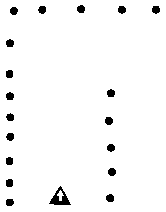
\includegraphics[width=\textwidth]{scanA.pdf}
		\caption{Scan 1}
		\label{fig:icp_scanA}
	\end{subfigure}
	\begin{subfigure}{0.12\textwidth}
		\centering
		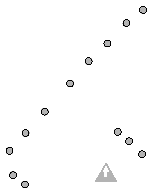
\includegraphics[width=\textwidth]{scanB.pdf}
		\caption{Scan 2}
		\label{fig:icp_scanB}
	\end{subfigure}
	\begin{subfigure}{0.20\textwidth}
		\centering
		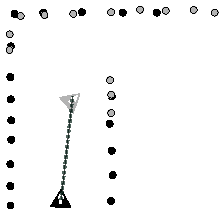
\includegraphics[width=\textwidth]{scanAB.pdf}
		\caption{Scans aligned}
		\label{fig:icp_scanAB}
	\end{subfigure}
	\caption{Proximity scan used to determine robot movement (transformation)}
	\label{fig:icp_scans}
\end{figure}

The basic ICP algorithm consist of the three following steps:
\begin{enumerate}
\item Construct correspondences between point set $\vec{p}$ and $\vec{q}$
\item Compute a transformation which minimizes the distances (errors) between the two correspondences
\item Apply the transformation to the set $\vec{p}$ and iterate until convergence
\end{enumerate}
A correspondence is a match between a point from set $\vec{p}$ and its nearest neighbour from set $\vec{q}$. 
Once the correspondences are found minimizing the error between them is stated in \eqref{eq:least_squares}.
Where $\mathbf{H}$ is a 2D homogeneous transformation matrix, $p_i$ is point $i$ from point set $\vec{p}$, $m_j$ is the closest point ($j$) from point set $\vec{q}$, $n_i$ is the normal vector to the line between the closest and second closest point in $\vec{q}$.
All points are in homogeneous coordinates.
\begin{equation}
\argmin_{\mathbf{H}} \sum_i ((\mathbf{H}p_i - m_j)n_i)
\label{eq:least_squares} 
\end{equation}
From \eqref{eq:least_squares} a linear system, $\mathbf{A}\vec{x}=\vec{b}$, is constructed and solved using QR-decompostion. The system is decomposed into $\mathbf{Q}$ and $\mathbf{R}$ using the Gramm-Schmidt method which is partially shown in~\eqref{eq:gram_schmidt}, where $\mathbf{A} = [\vec{v}_0,\vec{v}_1,\vec{v}_2,\vec{v}_3]$, and $\mathbf{Q} = [\vec{u}_0,\vec{u}_1,\vec{u}_2,\vec{u}_3]$.
\begin{equation}
\label{eq:gram_schmidt}
\begin{aligned}
\vec{u}_0 &= \frac{\vec{y}_0}{|\vec{y}_0|} \Rightarrow \vec{y}_0 = \vec{v}_0 \\
\vec{u}_1 &= \frac{\vec{y}_1}{|\vec{y}_1|} \Rightarrow \vec{y}_1 = \vec{v}_1 - (\vec{v}_1 \bullet \vec{u}_0)\vec{u}_0 \\
\vec{u}_2 &= \frac{\vec{y}_2}{|\vec{y}_2|} \Rightarrow \vec{y}_2 = \vec{v}_2 - (\vec{v}_2 \bullet \vec{u}_0)\vec{u}_0  - (\vec{v}_2 \bullet \vec{u}_1)\vec{u}_1 \\
%\vec{u}_3 &= \frac{\vec{y}_3}{|\vec{y}_3|} \Rightarrow \vec{y}_3 = \vec{v}_3 - (\vec{v}_3 \bullet \vec{u}_0)\vec{u}_0  - (\vec{v}_3 \bullet \vec{u}_1)\vec{u}_1 - (\vec{v}_3 \bullet \vec{u}_2)\vec{u}_2 \\
\end{aligned}
\end{equation}
The transformation $\vec{x}$ is retrieved by solving the system $\mathbf{R}\vec{x}=\mathbf{Q}^T \vec{b}$ where $\mathbf{R}$ is a $4 \times 4$ upper triangular matrix, a more detailed description is given in Chapter~5 and 12 of \cite{Robin:Hendrik}.

\subsection{Computing vectors to the closest points}

\lstset{basicstyle=\codesmall}

\begin{lstlisting}
icp :: SeqLogic s [Float] [Float] ()
icp = do
  vecPx <- receive
  clock
  vecPy <- receive
  clock
  vecQx <- receive
  clock
  vecQy <- receive
  clock

  vecNx <- alloc (replicate 180 undefined)
  vecNy <- alloc (replicate 180 undefined)
  vecMx <- alloc (replicate 180 undefined)
  vecMy <- alloc (replicate 180 undefined)

  loop 0 upto (180-1) $ \i -> do
    let px = vecPx!!i
    let vecDx = px -. vecQx
    clock
    let py = vecPy!!i
    let vecDy = py -. vecQy
    clock
    let vecDx2 = vecDx .*. vecDx
    clock
    let vecDy2 = vecDy .*. vecDy
    clock
    let vecSquaredDist = vecDx2 .+. vecDy2
    clock
    let (j,k) = indexSmallestTwo vecSquaredDist
    clock
    let mx0 = vecQx!!j
    let mx1 = vecQx!!k
    clock
    let my0 = vecQy!!j
    let my1 = vecQy!!k
    clock
    let (nx,ny)= findNormVec (px,py) (mx0,my0) (mx1,my1)
    clock
    vecMx?i <~ mx0
    clock
    vecMy?i <~ my0
    clock
    vecNx?i <~ nx
    clock
    vecNy?i <~ ny
\end{lstlisting}

\begin{lstlisting}
  v <- allocArr 4
  v0 <- peek vecNx
  v?0 <~ v0
  clock
  v1 <- peek vecNy
  v?1 <~ v1
  clock
  let v2'' = vecPx .*. v0
  clock
  let v2'  = vecPy .*. v1
  clock
  v?2 <~ v2' .+. v2''
  clock
  let v3'' = vecPx .*. v1
  clock
  let v3'  = vecPy .*. v0
  clock
  v?3 <~ v3'' .-. v3'
  clock
  vecMx' <- peek vecMx
  let b'' = vecMx' .*. v0
  clock
  vecMy' <- peek vecMy
  let b'  = vecMy' .*. v1
  clock
  let b   = b' .+. b''
\end{lstlisting}

\subsection{Solving a system of equations}

\begin{lstlisting}
  u <- allocArr 4
  call $ qr v u

  x <- allocArr 4
  linSolv <- start linearSolver
  loop 3 downto 0 $ \j -> do
     u_j <- peek (u?j)
     t_j <- inline $ u_j `dotProd` b
     infuse linSolv t_j
     loop 3 downto j $ \k -> do
        v_k <- peek (v?k)
        r_jk <- inline $ u_j `dotProd` v_k
        infuse linSolv r_jk
     x_j <- extract linSolv
     x?j <~ x_j
  finish linSolv
  
  transX <- peek (x?0)
  clock
  transY <- peek (x?1)
  clock
  cosTh <- peek (x?2)
  clock
  sinTh <- peek (x?3)
  clock
  let vecPxCt = cosTh *. vecPx
  clock
  let vecPySt = sinTh *. vecPy
  clock
  let vecPxCtPySt = vecPxCt .-. vecPySt
  clock
  let vecPx' = transX +. vecPxCtPySt
  clock
  let vecPyCt = cosTh *. vecPy
  clock
  let vecPxSt = sinTh *. vecPx
  clock
  let vecPyCtPxSt = vecPyCt .+. vecPxSt
  clock
  let vecPy' = transY +. vecPyCtPxSt
  clock

  emit (vecPx')
  clock
  emit (vecPy')
\end{lstlisting}

Solving the linear equations of an upper triangular matrix
\begin{lstlisting}
linearSolver :: SeqLogic s Float Float ()
linearSolver = do
  x <- allocArr 4
  loop 3 downto 0 $ \j -> do
     t_j <- receive
     tmp <- alloc t_j
     loop 3 downto (j+1) $ \k -> do
        r_jk <- receive
        x_k <- peek (x?k)
        let rx = r_jk * x_k
        clock
        t <- peek tmp
        tmp <~ t - rx
     r_jj <- receive
     t <- peek tmp
     let x_j = t / r_jj
     x?j <~ x_j
     emit x_j
  return ()
\end{lstlisting}

QR decomposition using the Gram�Schmidt process:
\begin{lstlisting}
qr :: Ref s [[Float]] -> Ref s [[Float]] ->
   SeqLogic s [Float] [Float] ()
qr v u = do
  loop 0 upto 3 $ \j -> do
     v_j <- peek (v?j)
     tmp <- alloc v_j
     loop 0 upto (j-1) $ \k -> do
        u_k <- peek (u?k)
        vj_uk <- inline $ v_j `project` u_k
        clock
        t <- peek tmp
        tmp <~ t .-. vj_uk
     t <- peek tmp
     u_j <- inline $ normalize t
     u?j <~ u_j
  return ()
\end{lstlisting}

\begin{lstlisting}
indexSmallestTwo :: [Float] -> (Int, Int)
indexSmallestTwo distances = (j,k) where
  ids = zip distances [0..]
  (xs, ys) = splitAt (div (length distances) 2) ids
  sortedLayer = zipWith sortTwo xs ys 
  (_,j,_,k) = foldl1 combineSmallestPairs sortedLayer

--sort two points, output is (y, iy, z, iz) where y < z
sortTwo :: (Float,i) -> (Float,i) -> (Float,i, Float,i)
sortTwo (a, ia) (x, ix) 
  | a < x   = (a, ia, x, ix)
  | otherwise = (x, ix, a, ia) 

--find the two closest distances out of two pairs 
--NOTE: assume input tuples are sorted (a < b && x < y)
combineSmallestPairs :: (Float, i, Float, i) ->
   (Float, i,  Float, i) -> (Float, i, Float, i)
combineSmallestPairs (a, ia, b, ib) (x, ix, y, iy) =
  case (a < x, b < x, a < y) of 
    (True, True, _)   -> (a, ia, b, ib)
    (True, False, _)  -> (a, ia, x, ix)
    (False, _, True)  -> (x, ix, a, ia)
    (False, _, False) -> (x, ix, y, iy)
\end{lstlisting}

Some multi cycle helper functions working with vectors; normalisation, dot product and vector projection:
\begin{lstlisting}
normalize :: [Float] -> SeqLogic s i o [Float]
normalize xs = do
   let sqs = xs .*. xs
   clock
   let n = sum sqs
   clock
   let invsq = invSqrt n
   clock
   return (invsq *. xs)

dotProd :: [Float] -> [Float] -> SeqLogic s i o Float
dotProd xs ys = do
   let zs = xs .*. ys
   clock
   return (sum zs)

project :: [Float] -> [Float] -> SeqLogic s i o [Float]
project vs us = do
   let zs = vs .*. us
   clock
   let n = sum zs
   clock
   return (n *. us)
\end{lstlisting}

For convenience we define operators for scalar-vector and vector-vector operations:
\begin{lstlisting}
n *. xs = map (n*) xs
n +. xs = map (n+) xs
n -. xs = map (n-) xs
(.*.) = zipWith (*)
(.+.) = zipWith (+)
(.-.) = zipWith (-)
\end{lstlisting}

\lstset{basicstyle=\codefamily}

\subsection{Comparison with manual designed hardware}
\begin{itemize}
  \item some remarks about the differences between the implementations and effort from hardware designer
  \item compare hardware implementation with the generated results from this section
\end{itemize}  

\textit{Work in progress}

\subsection{Optimizing the ICP implementation}
\begin{itemize}
  \item Apply software pipelining to speed up the finding of nearest two points loop.
  \item Use an ALU output register and computation reordering to limit the data memory usage to a single read port.
\end{itemize}  

\textit{Work in progress}


\section{Generating a processor}
\begin{itemize}
  \item source to source transformation using Haskell-src-exts parser
  \item input sequential logic edsl, output clash subset of haskell
\end{itemize}

\textit{To be extended}

\subsection{Resource requirement analysis}
The first step is to find for each cycle which variables are used and which are defined and used in another cycle.
This determines the amount of read and write ports required on the data memory, and how many inputs and outputs the ALU structure needs.
We need to take the type of variables in account, as variables of different size may need to be stored in different memories. \\

\textit{To be extended}

\subsection{Dealing with control flow}
\begin{itemize}
  \item side effect free if expressions within a cycle just become part of an alu instruction \\
  \item problems with delays in the control path
  \item control unit keeps track of loop counters to support zero overhead loop constructs
\end{itemize}

\textit{To be extended}

\subsection{Memory structure and addressing}

\begin{itemize}
  \item how to emulate multiport memories with blockram
  \item local variables are addressed relative to the stack pointer
  \item explicit allocated memory is addressed absolutely, thus not allowed in recursion functions
  \item every read and write port gets its own address generation unit (AGU) with access to the loop counters
  \item if a part of a memory element is written in a program then the memory is split in parts with a writemask to control them
\end{itemize}

\textit{To be extended}

\subsection{Optimise timing and reuse}
\begin{itemize}
  \item memory with read delay to better match with hardware
  \item ALU output registers with bypass for higher clocks?
  \item common subexpression detection on alu expressions
\end{itemize}

\subsection{Generating \clash code}
\begin{itemize}
  \item each (co)processor in its own file
  \item all declarations except for the sequential logic functions are copied
\end{itemize}

\textit{To be extended}


\subsection{Hardware tradeoffs}
The design of processors and mapping of algoritm involves many tradeoffs beyond deciding what happens in which cycle:
\begin{itemize}
  \item storing data in registers vs. data stack memory
  \item direct control versus using an instruction memory
  \item where do constants come from?
  \item extra delay (pipeline register) before or after the ALU to increase clock frequency
\end{itemize}
We would like to provide some options in our compiler to control those choices in the generated hardware. \\

\textit{Work in progress}


\section{Related approaches}

Using Haskell EDSLs to generate efficient low level code is common approach to gain both abstraction and performance, Feldspar \cite{Feldspar} (used for generating C code for digital signal processing) is a nice example of this.
Going from functional program descriptions to physical hardware realisation using Geometry of Synthesis \cite{Ghica} is different in many aspects, although it has similar goals. \\
%Cryptol??
%Copilot??

\textit{To be extended}

\subsection{High level synthesis}
Generates hardware from software written in ordinary programming languages (commonly C(++) or Matlab).
We could describe our process as medium level synthesis, because with explicit clock cycle boundaries we do not have to select and schedule operations.
While most high level synthesis approaches start from a behavioural description of an algorithm and have to deal with multiple hard optimisation problems. \\

\textit{To be extended}

\subsection{Customisable processors}
Starting with a template of a processor to which specialised ALUs and/or coprocessors to accelerate specific algorithms. \\
% No instruction set processor

\textit{To be extended}


\section{Conclusions}

A processor is a thing that executes programs in many bounded steps.
Merely defining the boundaries of steps to execute and their ordering is enough to derive processor like hardware structure from it. \\

\textit{To be extended}

%Instruction set design can be systematic refactoring process \\
%The program and hardware constraints drive the steps to take \\
%Besides minor optimizations only a few design choices to make \\
%As a side effect derived instruction set are easy to compile for


\subsection{Future work}
Implement the transformation process as GHC plugin instead of a fragile source to source compilation.
Or even better convince the \clash developers to integrate this transformation process in their compiler, as that gives access to more information about the hardware to be generated.

Find suitable higher level abstractions to make the EDSL more functional than the current imperative features.

Would it be possible to extend the work of 'Calculating Correct Compilers' \cite{CCC} to derive both a compiler and processor? \\

\textit{More to be added}

% Start from language semantics instead of specific programs \\
% Extend for other language features (memory/complex control flow) \\
% Automating parts of the process or better refactoring tools\\
% Work out the process for pipelining and data parallelism? 


\begin{acks}
The first author conducted this research within the Modern project (647.000.003) supported by NWO.
\end{acks}

\bibliography{p2p}

\end{document}
